%%%%%%%%%%%%%%%%%%%%%%%%%%%%%%%%%%%%%%%%%%%%%%%%%%%%%%%%%%%
%
%        
%
%\documentclass[letterpaper, 10 pt, conference]{ieeeconf}  % Comment this line out if you need a4paper
%
\documentclass[a4paper, 10pt, conference]{ieeeconf}      % Use this line for a4 paper
%
%\IEEEoverridecommandlockouts                              % This command is only needed if 
                                                          % you want to use the \thanks command
%
\overrideIEEEmargins                                      % Needed to meet printer requirements.
%
% See the \addtolength command later in the file to balance the column lengths
% on the last page of the document
%
\usepackage{graphicx} % for pdf, bitmapped graphics files
%\usepackage{hyperref}
%\hypersetup{colorlinks,urlcolor=blue,linkcolor=blue}
%
\usepackage{epstopdf}
%\usepackage{mathptmx} % assumes new font selection scheme installed
%\usepackage{times} % assumes new font selection scheme installed
\usepackage{amsmath} % assumes amsmath package installed
\usepackage{amssymb}  % assumes amsmath package installed
\usepackage{graphicx}
%\usepackage{subfig}
\usepackage{caption}
\usepackage{subcaption}
\usepackage{array}
\usepackage[space]{cite}
%\usepackage[hidelinks]{hyperref}
\usepackage[colorlinks, linkcolor = black, citecolor = black, filecolor = black, urlcolor = blue]{hyperref}
\usepackage{lscape} %% landscape
\usepackage{longtable} %% big table
\usepackage{tikz}

\newcommand\encircle[1]{%
	\tikz[baseline=(X.base)] 
	\node (X) [draw, shape=circle, inner sep=0.5pt] {#1};}





%\DeclarePairedDelimiter\abs{\lvert}{\rvert}%
%\DeclarePairedDelimiter\norm{\lVert}{\rVert}%
\DeclareMathOperator*{\argmin}{argmin}
\DeclareMathOperator*{\argmax}{argmax}
\DeclareMathOperator*{\sgn}{sgn}
\newcommand{\specialcell}[2][c]{%
	\begin{tabular}[#1]{@{}c@{}}#2\end{tabular}}

\renewcommand{\citedash}{--}


\newcommand{\etal}{~\textit{et al.}}
%
\title{\bf {\LARGE Mechanisms and Sensors for Robotic Fingers} \\
{\normalsize H$^2$T-Seminar: Humanoid Robotics, WS 18/19}}
\author{Shant Gananian, Pascal Weiner and Tamim Asfour \\ High Performance Humanoid Technologies \\ Institute for Anthropomatics and Robotics \\ Karlsruhe Institute of Technology \\
\url{http://www.humanoids.kit.edu}}


%
%
\begin{document}
\maketitle
\thispagestyle{empty}
\pagestyle{empty}
%
%%%%%%%%%%%%%%%%%%%%%%%%%%%%%%%%%%%%%%%%%%%%%%%%%%%%%%%%%%%%%%%%%%%%%%%%%%%%%%%%
\begin{abstract}
: Grasping is achieved in robots by suitable finger mechanisms inspired from structures in nature. This paper discusses anthropomorphic fingers, their actuators and sensors, their characteristics and operation of their mechanisms.
\end{abstract}

%%%%%%%%%%%%%%%%%%%%%%%%%%%%%%%%%%%%%%%%%%%%%%%%%%%%%%%%%%%%%%%%%%%%%%%%%%%%%%%%
\section{\textbf{Introduction}}
The first robotic hand, as it is commonly referred to, was perhaps the end-effector of the Handyman, a robot developed by Ralph Mosher for General Electric in 1960. Around 1969, the first research projects on robotic hands with three fingers including a “thumb” in opposition—hence an anthropomorphic design—began in the United States and in Japan.\\
The idea of copying the human hand is so old and may be contemporary of the first automata in the 18th century, e.g., La Musicienne of the inventor Jacquet-Droz (Rosheim 1994). This automate was able to play a wide variety of organ partitions with two five-finger hands actuated with steel cables connected to a programming cam shaft.\\
For a prosthetic hand the focus is much more on aesthetics, weight and broad range of functionality, while the supply of power is limited, so self-locking mechanisms are preferred. Today’s prosthetic hands have integrated drive technologies and weigh less than 500 g.\\
Because of the dexterity of the human hand, most recent humanoid robots research projects addressed in their designs the anthropomorphism of the robotic hand. Many research laboratories around the world have developed prototypes of such hands as early as in the mid 1980’s when the foundations of these studies were laid (Mason and Salisbury 1985), by taking the human hand as a model for the robotic manipulation, in terms of performance and versatility. But results thus far are not comparable with the performances of the human hand.\\
Anthropomorphism is the capability of a robotic end-effector to mimic the human hand.\\
Dexterity is the ability to autonomously perform highly precise operations with a certain level of complexity (visual/perceptual/tactile feedback).  The dexterity domain can be divided in two main areas, grasping (grasped object is fixed with respect to the hand workspace) and internal manipulation (controlled motion of the grasped object inside the hand workspace).\\
The dexterity of robots has always been clearly more limited than that of a well-trained human being.\\
In fact we can find anthropomorphic end-effectors with very poor dexterity level, even if they are called hands, they perform very rough grasping procedures. Similarly, we can find smart end-effectors, capable of sophisticated manipulation procedures, but without any level of anthropomorphism.\\
Anthropomorphism is not necessary for achieving dexterity, and nor sufficient. But still it is desirable goal in the design of robotic end-effectors in operating in an environment where tasks may be executed by a robot or by a man, or in tele-operation of the end-effector by a man, or when it is required that the robot has human-like aspects and behavior.\\
Considering that the human hand is capable of prehension (grasping objects of different size and shape) and apprehension (understanding through active touch), then it is both an output and input device. It can apply forces and provide information about the state of the interaction with the object. These characteristics are desirable in advanced robot hands.\\
The average human hand is around 0.58\% of total body weight (approximately 400g).\\
Human hands have a highly articulated thumb. Amputation of the thumb is cited to cause 40\% loss of hand function and around 20\% disability of the whole person. The main motions of the thumb are flexion, extension, abduction/adduction and opposition. The thumb facilitates the grasping tasks by means of these motions.\\
%%%%%%%%%%%%%%%%%%%%%%%%%%%%%%%%%%%%%%%%%%%%%%%%%%%%%%%%%%%%%%%%%%%%%%%%%%%%%%%%
\section{\textbf{Robotic Fingers}}
Fingers of the hand are organs of manipulation and sensation. They move in the following ways: flexion, extension, abduction and adduction.\\
The number of joints per finger in anthropomorphic robotic hands is extremely important since it provides the hand with conformance to shapes and acts as a contact surface for gripping and support structure for grasps.\\
Number of fingers in anthropomorphic robotic hands can differ, but increased number of fingers provide a larger grasping surface and increases conformity to shapes.\\
The anatomy of fingers in nature shows us the following design characteristics:\\
\begin{itemize}
	\item A serial bone-link structure mainly for rigidity and load capability.
	\item An actuation muscle system aiming to rotate each bone-link independently but with coordinate movements with other finger links.\\
\end{itemize}
%%%%%%%%%%%%%%%%%%%%%%%%%%%%%%%%%%%%%%%%%%%%%%%%%%%%%%%%%%%%%%%%%%%%%%%%%%%%%%%%
\section{\textbf{Requirements for Artificial Fingers}}
In general common requirements can be identified mainly in the aspects for:\\
\begin{enumerate}
  \item Motion properties in:
  	\begin{itemize}
  		\item Grasping configurations
  		\item Smooth approaching motion
		\item Adaptable motion configuration to object shapes
		\item Reconfigurable grasping configurations
		\item Workspace ranges
		\item Limited motion impacts again objects to be grasped
	\end{itemize}
  \item Force capability in:
  	\begin{itemize}
  		\item Stable grasping configurations
		\item Efficient transmission of input power to grasping forces
		\item Distribution of grasping forces among several contacts with grasped object
		\item Positions of application points of the grasping forces
		\item Adjustable grasping forces
  	\end{itemize}
  \item Mechanical design in:
  	\begin{itemize}
  		\item Stiff or compliant structure at grasp
		\item Phalanx shape for adaptability to object shape
		\item Room for sensors
		\item Compact design versus human-like solutions
		\item Lightweight solution with smart or traditional materials
		\item Low-friction joints
		\item Location of power source\\
  	\end{itemize}
\end{enumerate}
A general procedure can be outlined as in Fig.\ref{fig:design1}.
\begin{figure}[h!]
\centering
  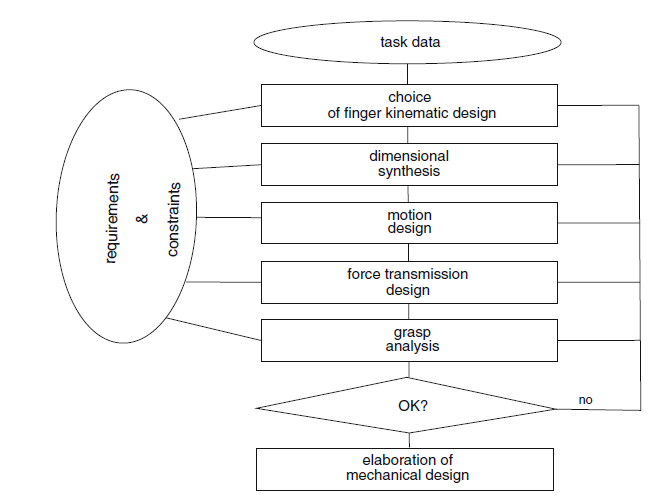
\includegraphics[width=0.7\linewidth]{./images/design}
  \caption{A flowchart for design procedure of finger mechanisms}
  \label{fig:design1}
\end{figure}

%%%%%%%%%%%%%%%%%%%%%%%%%%%%%%%%%%%%%%%%%%%%%%%%%%%%%%%%%%%%%%%%%%%%%%%%%%%%%%%%
\section{\textbf{Actuators}}
Human hands vary greatly in their speed and grip force and are capable of reaching up to 400 N in everyday tasks. This kind of actuation characteristics is not achievable with the current motors available in the market, considering them to be situated in the hand. For that reason remote actuation is used in many cases, for example by placing actuators in the forearm and using tendons to transmit the forces to the finger joints.\\
For developing anthropomorphic finger mechanisms researches used two different approaches: complex mechanisms for performing manipulation tasks with high dexterity, or mechanisms with a reduced number of degrees of freedoms (DoFs) and actuators.\\
\begin{enumerate}
  \item \textbf{Level of actuation:}
Aside from the number of fingers and number of joints per finger, robotic hands can be distinguished by their level of actuation.\\
 	\begin{itemize}
 		\item fully actuated: every joint is independently controllable DoF = DoC
 		\item under actuated: some of the joints are coupled mechanically DoF > DoC\\
 	\end{itemize}
Underactuated hands are preferred by designers because of the reduction of required actuators which affects the size, the weight and the complexity of the hand. This also makes the control of the system simpler.\\
  \item \textbf{Type of actuation:}
Actuators and transmissions used in robotic hands can be:\\
	\begin{itemize}
		\item electric motors
		\item pneumatic actuators
		\item hydraulic actuators
		\item shape memory alloys (SMA)\\
	\end{itemize}
Despite the electric motors represent the choice with smallest power density it is the most common solution adopted in the development of robotic hands. This is compensated by the flexibility and simplicity of the control, and the wide availability of the batteries.\\
Pneumatic actuators have high power density, but low stiffness, and that makes the control complicated. The energy required has to be stored in a tank (big volumes), the system needs compressor, pressure sensors and regulator. All these components take a quite a bit of valuable space and are quite expensive.\\
Hydraulic actuators have very high performance indices but have the same storage difficulties of pneumatic actuators, and they are hard to miniaturize because they need to work with high pressures.\\
The shape memory alloys (SMA) are materials that have the ability to contract when heated above a certain temperature allowing muscle-like movements. They are very compact, totally silent and when contracting exhibit ample forces. Consequently, they can be successfully used for driving dexterous prosthetic hands.\\
One major disadvantage is their response speed which is relatively slow being limited by the speed with which the SMA can be heated and cooled. Other disadvantages are the power requirements, control difficulties and the limited internal space. This technology seems to be not mature yet.\\
  \item \textbf{Type of transmission:}
The mechanism for transmitting the motor power to the joints could be categorized as:\\
\begin{itemize}
		\item tendon and pulleys or sheath, like steal wires, synthetic strings, plastic strips
		\item link transmission (rigid connection), like gears, articulated mechanism\\
	\end{itemize}
Using tendons to transmit the power to the joint shaft allows us to place the actuators remotely. It also allows us to reduce the number of parts required for the linkage.\\
The classical geared coupling mechanisms add weight to the device but offer better performance in terms of friction. It is a good solution especially when we are limited with the available space and actuators have to be integrated in the palm of the hand or in the fingers.\\
\end{enumerate}
%%%%%%%%%%%%%%%%%%%%%%%%%%%%%%%%%%%%%%%%%%%%%%%%%%%%%%%%%%%%%%%%%%%%%%%%%%%%%%%%
\section{\textbf{Sensors}}
Sensors play a major role in anthropomorphic robotic hands. They are what robotic systems use to get useful data of its own state or the environment around it. Some of the key types of sensors are:\\
	\begin{itemize}
	\item \textbf{Joint / Position sensors:} They give feedback on the link and joint position in the robot’s workspace. In underactuated hands, it also provides feedback on the grasp and its conformity with the shape of the object being handled.\\
	\item \textbf{Force / Torque sensors:} To get information on the amount of the force being applied by the hand on the environment and the forces and torques that are present within the system itself.\\
	\item \textbf{Tactile / Touch sensors:} As proposed by Yousef, H. et al. [9] the minimum functional requirements for a robotic tactile sensing system mimicking human manipulation is summarized as:\\
		\begin{itemize}
			\item Detect the contact and release of an object.
			\item Detect lift and replacement of an object.
			\item Detect shape and force distribution of a contact region for object recognition.
			\item Detect contact force magnitude and direction for maintaining a stable grasp during manipulation.
			\item Detect both dynamic and static contact forces.
			\item Track variation of contact points during manipulation.
			\item Detect difference between predicted and actual grip forces necessary for manipulation.
			\item Detect force and magnitude of contact forces due to the motion of the hand during manipulation.
			\item Detect tangential forces due to the weight and shape of the object to prevent slip.
			\item Detect tangential forces arising from variations in object parameters (e.g. surface friction, elasticity, etc.) to prevent slip.\\
		\end{itemize}
	\item \textbf{Other sensors:} temperature, olfactory, vision, depth sensing, stress, strain, twist etc.\\
	\end{itemize}
The skin of human body is covered with a continuous network of tactile sensors offering feedback about the amount of force applied and the region the force is applied to, within a threshold.\\
The skin temperature can assist in identifying the object while grasping especially when there is no visual feedback (trying to grasp in the dark).\\
Cameras could be integrated on the palm and fingers of robotic hands, therefore making it possible to have a wide view when far away and high resolution when close up, with the freedom to actively avoid occlusions.\\

\begin{landscape}
\begin{table}[]
\centering
\caption{Hand comparison chart from 1983 to 2016.}
\label{my-label}
\begin{tabular}{p{2cm}p{4cm}lp{2cm}p{2cm}lllp{2cm}lll}
\hline
\multicolumn{1}{c}{\textbf{Name}} & \multicolumn{1}{c}{\textbf{Sensors}} & \multicolumn{1}{c}{\textbf{Fingers}} & \multicolumn{1}{c}{\textbf{Transmission}} & \multicolumn{1}{c}{\textbf{Research Institute}} & \multicolumn{1}{c}{\textbf{Year}} & \multicolumn{1}{c}{\textbf{DOF}} & \multicolumn{1}{c}{\textbf{DOA}} & \multicolumn{1}{c}{\textbf{Actuators}} & \multicolumn{1}{c}{\textbf{Weight {[}Kg{]}}} & \multicolumn{1}{c}{\textbf{Load {[}Kg{]}}} & \multicolumn{1}{c}{\textbf{Load {[}N{]}}} \\ \hline
Stanford/JPL Hand & Tactile Sensors, Tension tendons sensors & 3 & Tendons & Stanford University & 1983 & 9 & 9 & Electrical (DC) & 1.1 &  & 110.8 \\ \hline
Utah/MIT & Hall effect sensors, Tendon tension sensors, tactile distributed sensors & 4 & Tendons & Utah University & 1985 & 16 & 16 & Pneumatic Cylinders & 9 & 9 &  \\ \hline
Belgrade/USC Hand & Potentiometers as positions sensors, Force resistors & 5 &  & Belgrade University & 1988 & 15 & 4 & Electrical Motors &  & 2.26 &  \\ \hline
BarrettHand & Optical Encoders, Tactile sensors & 3 & Tendons, worm gears & Barret Technology Inc. & 1988 & 8 & 4 & Electrical Brushless motors & 1.2 & 6 &  \\ \hline
DLR Hand I & 28 Sensors on each finger, hall sensors, optical position sensor, torque sensor, force sensor, tactile sensors and stereo camera & 4 & Tendons & DLR-German Aerospace Center & 1997 & 16 & 12 & Electrical &  &  &  \\ \hline
Dist Hand & Rotation sensors in each joint & 5 & Tendons & Genova University & 1998 & 16 & 16 & Electrical & 1 &  & 1.96 \\ \hline
Robonaut Hand & 42 sensors plus tactile sensors & 5 & Tendons & NASA Johnson Space Center & 1999 & 19 & 14 & Electrical Brushless Motors &  & 9 &  \\ \hline
Gifu Hand & Magnetic encoder in the motors shaft and tactile distributed sensor & 5 & Gears , Links & Gifu University & 1999 & 20 & 16 & DC Micromotors & 1.4 & 1.83 &  \\ \hline
Robotiq 3 Finger Gripper & current sensor, position sensor, grip sensor & 3 & gears and links & Laval University & 1999 & 10 & 4 & DC Motors & 2.3 & 10 &  \\ \hline
Blackfingers & Position and force sensors directly on the actuator & 5 & Tendons & Politecnico de Milano & 2000 & 22 & 36 & Mckibben Actuators &  &  &  \\ \hline
\begin{tabular}[c]{@{}l@{}}Tuat/Karlsruhe\\   Hand\end{tabular} &  & 5 & Tendons & Tokyo and Karlsruhe Universities & 2000 & 24 & 1 & Electrical & 0.49 &  &  \\ \hline
Ultralight Hand &  & 5 & NONE & Research Center of Karlsruhe & 2000 & 18 & 13 & Flexible Fluidic actuators & 0.2 & 1.22 &  \\ \hline
Variable Force Hand &  & 5 & Tendons & Hokkaido University & 2000 & 10 & 5 &  &  &  &  \\ \hline
DLR Hand II & Torque sensors in each joint & 4 & Tendons & DLR-German Aerospace Center & 2001 & 17 & 13 & Electrical & 2.2 & 3.059 &  \\ \hline
RTR Hand I & Hall effect sensors, strain gages as force sensors & 3 & Screws & Centro INAIL RTR, Scuola Superiore Santa Anna & 2001 & 9 & 3 & DC Micromotors &  &  &  \\ \hline
Dexterous Robot &  & 4 & Tendons & Maryland University & 2001 & 12 &  &  &  &  &  \\ \hline
Shadow EDC Hand & Hall effect sensors, Tactile sensors & 5 & Tendons & Robot Shadow Company Ltd. & 2002 & 23 & 23 & Pneumatic muscles & 4 &  &  \\ \hline
Thinh Hand & Bend Sensors, Camera for visual control of the thumb pronation angle & 4 & Tendons & Florida University & 2002 & 14 & 6 & Electrical &  &  &  \\ \hline

\end{tabular}
\end{table}
\end{landscape}

\begin{landscape}
\begin{table}[]
\centering
\caption{(Continued).}
\label{my-label}
\begin{tabular}{p{2cm}p{4cm}lp{2cm}p{2cm}lllp{2cm}lll}
\hline
\multicolumn{1}{c}{\textbf{Name}} & \multicolumn{1}{c}{\textbf{Sensors}} & \multicolumn{1}{c}{\textbf{Fingers}} & \multicolumn{1}{c}{\textbf{Transmission}} & \multicolumn{1}{c}{\textbf{Research Institute}} & \multicolumn{1}{c}{\textbf{Year}} & \multicolumn{1}{c}{\textbf{DOF}} & \multicolumn{1}{c}{\textbf{DOA}} & \multicolumn{1}{c}{\textbf{Actuators}} & \multicolumn{1}{c}{\textbf{Weight {[}Kg{]}}} & \multicolumn{1}{c}{\textbf{Load {[}Kg{]}}} & \multicolumn{1}{c}{\textbf{Load {[}N{]}}} \\ \hline
High Speed Multifingered Hand & Strain gages, Camera for image processing & 3 & Miniharmonic drive, bevel gears & Tokyo and Hiroshima Universities & 2003 & 10 & 10 & Electrical & 0.8 & 2.85 &  \\ \hline
SMA Hand & Planed to have Position Sensors, Force Sensors and Touch Sensors & 4 & Shape Memory Alloy Wires & State University of New Jersey & 2004 & 14 &  & Electrical & 1.3 & 3.6 &  \\ \hline
ARMAR Hand & Angle sensors, Force Sensors and Pressure Sensors & 5 & Flexible Fluidic Actuators & University of Karlsruhe & 2005 & 8–18 & 8–16 & Micro Gear Pump & 0.49 & 11.21 &  \\ \hline
UB Hand III v1 & Strain=gauge based sensors, position sensors, tendon force sensors & 5 & Elastic Hinges with Tendons & University of Bologna & 2005 & 20 & 16 & DC Brushed Motors &  &  &  \\ \hline
RL1 Hand & Tendon Tension through mathematical approximation & 3 & Tendons & Universidad Carlos III de Madrid & 2006 & 8 & 1 & DC Motors & 0.25 & 2 &  \\ \hline
AAA Hand & External optotrank (Infrared optical device) & 3 & Tendons & Scuola Superiore Santa Anna & 2007 & 10 & 4 & DC Motors & 0.25 & 3.56 &  \\ \hline
FRH-4 Hand & Position Sensors, Tactile Sensors & 5 & Flexible Fluidic Actuators & Research Center Karlsruhe & 2008 & 11 & 12 & Gear Pump & 0.216 & 11.21 &  \\ \hline
IH2 Azzurra & Tendon Force Sensors, 2 Axis fingertip force sensor & 5 & Tendons & Prensilia & 2008 & 11 & 5 & Electric Motors & 0.6 & 10.2 &  \\ \hline
UB Hand III v2 & Optical angular sensors, Optical Tensor Sensors, Strain gauge tension sensors & 5 & Tendons & Bologna University & 2009 & 20 &  & Mckibben Artificial Muscles &  &  &  \\ \hline
TH-3R Hand &  & 5 & Gears, Racks & Tsinghua University & 2009 & 15 & 4 & Motors &  &  &  \\ \hline
Columbia Hand & Position Sensors, Tactile Sensors & 3 & Tendons & Columbia University & 2011 & 9 & 2 & Motors &  &  &  \\ \hline
The Handroid &  & 5 & Tendons & ITK Company & 2011 & 16 & 5 & DC Motors & 0.725 &  &  \\ \hline
KYTECH Hand & Position Sensor & 4 & Gears & Korea Institute of Industrial Technology & 2012 & 16 & 16 & DC Motors & 0.9 & 1.5 &  \\ \hline
The PISA/IIT Soft Hand &  & 5 & Tendons, Rolling cylinders & University of Pisa & 2012 & 18 & 1 & Electric Motor &  &  &  \\ \hline
TDM Hand & No sensors, force approximation using Ozawa and Moriya technique & 3 & Tendons & Ritsumeikan University & 2013 & 12 & 12 & DC Motors &  & 5.1 &  \\ \hline
iHY Robot Hand & Pressure sensors, Optic sensors & 3 & Tendons & Yale and Harvard University & 2014 & 9 & 5 & DC Motors &  & 22 &  \\ \hline
Soft Robotic Hand & Resistive Bend sensors & 3 & Pneumatic tubing & Massachusetts Institute of Technology & 2015 &  &  & Pneumatic piston &  &  &  \\ \hline
HALS &  & 5 & Tendon & Yokohama National U & 2016 & 9 & 5 & DC Motor & 1.2 & 3.059 &  \\ \hline
RBO Hand 2 &  & 5 & Pneuflex & Berlin University of Technology & 2016 & 5 & 7 & Pneumatic & 0.178 & 0.5 &  \\ \hline
UW’s Hand & Joint and Tactile Sensors & 5 & Tendons & University of Washington & 2016 &  & 10 & Servo Motors & 0.942 &  &  \\ \hline
\end{tabular}
\end{table}
\end{landscape}

\listoffigures
\bibliography{./References}
\bibliographystyle{./IEEEtran}
\nocite{*}

%
\end{document}
%
